\begin{theo}[Wederzijdse inductie]{Wederzijdse inductie}
    \begin{minipage}{.78\textwidth}
        Als twee spoelen nabij elkaar plaatst worden, zoals in de figuur, dan zal een veranderende stroom in de ene, 
        een emf induceren in de andere. Dus: geïnduceerde emf in een spoel is enevredig met de snelheid van de stroomverandering
        in de andere. Dit noemt men \textbf{wederzijdse inductie} $M$, we noteren
        \begin{equation*}
            M_{21} = \dfrac{N_{2}\Phi_{21}}{I_{1}} 
        \end{equation*}
        met $M_{21}$ de wederzijdse inductiecoefficient en $\Phi_{21}$ de magnetische flux doorheen spoel 2 tegenover de stroom in spoel 1.
        We kunnen dit mengen met de wet van Faraday
    \end{minipage}
    \begin{minipage}{.18\textwidth}
        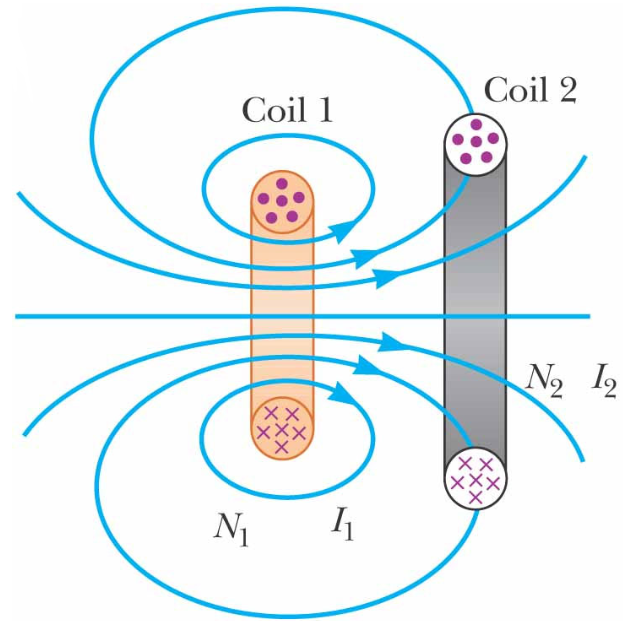
\includegraphics[scale=0.3]{Images/Magnetisme/WederzijdseInductie}
    \end{minipage}
    \begin{equation*}
        \mathcal{E}_{2} = - N_{2}\dfrac{d\Phi_{21}}{dt} = - M_{21}\dfrac{dI_{1}}{dt}
    \end{equation*}
    waarbij nu de verandering in stroom in spoel 1 hebben verbonden aan de emf dat het induceert in spoel 2.  In de algemene situatie is 
    $M = M_{12} = M_{21}$.
\end{theo}

\begin{app}[Wederzijdse inductie van een solenoïde en een spoel]{Wederzijdse inductie van een solenoïde en een spoel}
    De solenoïde is opeengepakt, dus kunnen we veronderstellen dat alle magnetische flux in de solenoïde blijft in de tweede spoel.
    We weten dam wat de flux door deze spoel is, namelijk
    \begin{equation*}
        \Phi_{21} = BA = \mu_{0}\dfrac{N_{1}}{\ell}I_{1}A
    \end{equation*}
    en de wederzijdse inductiecoëfficient
    \begin{equation*}
        M = \dfrac{N_{2}\Phi_{21}}{I_{1}} = \mu_{0}\dfrac{N_{1}N_{2}}{\ell}A
    \end{equation*}
    waarbij we zien dat deze enkel afhangt van de geometrie van het systeem.
\end{app}

\begin{theo}[Zelfinductie]{Zelfinductie}
    De magnetische flux $\Phi_{B}$ door een spoel met $N$ windingen (of eenderwelke kring) is evenredig met de stroom $I$ die erdoor vloeit, dus we definiëren de \textbf{zelfinductie} $L$ als
    \begin{equation*}
        L = \dfrac{N\Phi_{B}}{I}
    \end{equation*}
    Dus de geïnduceerde emf $\mathcal{E}$ in een spoel met zelfinductie $L$ is, volgens de wet van Faraday, gelijk aan
    \begin{equation*}
        \mathcal{E} = -N\dfrac{d\Phi_{B}}{dt }= - L\dfrac{dI}{dt}
    \end{equation*}
    \vspace{-0.3cm}
\end{theo}

\newpage

\begin{theo}[Energie opgeslagen in een magnetisch veld]{Energie opgeslagen in een magnetisch veld}
    Wanneer een inductor met zelfinductie $L$ een stroom $I$ heeft, die verandert met een snelheid $dI/dt$, dan is de energie die 
    gelever wordt aan de inductor gelijk aan 
    \begin{equation*}
        P = \mathcal{E}I = -LI\dfrac{dI}{dt}
    \end{equation*}
    De hoeveelheid arbeid $dW$ geleverd aan de inductor in een tijd $dt$ is gelijk aan
    \begin{equation*}
        dW = Pdt = -LIdI
    \end{equation*}
    De energie die opgeslagen is in het magnetisch veld van de inductor is gelijk aan de energie die geleverd is aan de inductor
    \begin{equation*}
        U = \int dW = \int Pdt = \int_{0}^{I} -LIdI = \dfrac{1}{2}LI^{2}
    \end{equation*}
    wat heel vergelijkbaar is aan de formule voor de energie opgeslagen in een condensator, namelijk: $U_{C} = \frac{1}{2}C(\Delta V)^{2}$. 
    Net zoals de energie in een condensator zich bevindt in het elektrisch veld tussen de platen,bevindt de energie in een inductor zich in het magnetisch veld binnenin de spoel.
\end{theo}

\begin{app}[RL-kringen]{RL-kringen}
    \vspace{-0.5cm}
    \begin{minipage}{.66\textwidth}
        We sluiten de schakelaar en we passen de tweede wet van Kirchhoff toe op de kring. We krijgen
        \begin{equation*}
            V_{0} - IR - \mathcal{E} = V_{0} - IR - L\dfrac{dI}{dt} = 0
        \end{equation*}
        We kunnen dit herwerken tot een differentiaalvergelijking
        \begin{equation*}
            L\dfrac{dI}{dt} + RI = V_{0}
        \end{equation*}
        wat we oplossen tot 
        \begin{equation*}
            I(t) = \dfrac{V_{0}}{R}\left(1 - e^{\tfrac{-t}{\tau}}\right)
        \end{equation*}
    \end{minipage}
    \begin{minipage}{.3\textwidth}
        \hspace{0.5cm}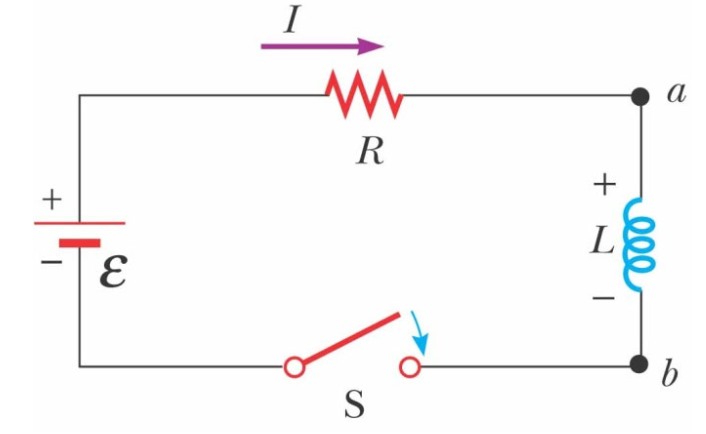
\includegraphics[scale = 0.35]{Images/Magnetisme/RLKring}
        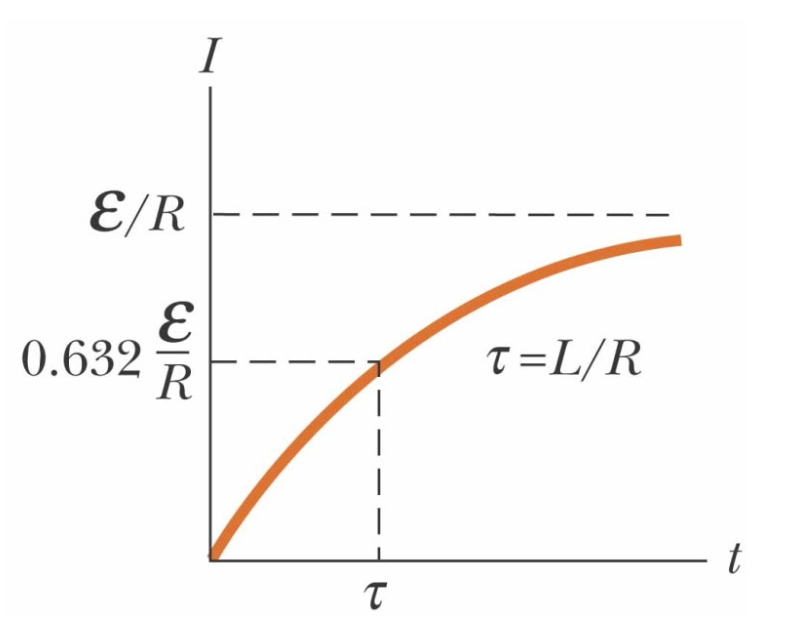
\includegraphics[scale = 0.35]{Images/Magnetisme/RLKringGraph.png}
    \end{minipage}

    \noindent met $\tau = \tfrac{L}{R}$. We zien dat de stroom initieel snel stijgt en dan afvlakt geleidelijk nabij $\tfrac{\mathcal{E}}{R}$.
\end{app}
